\documentclass{beamer}
\usetheme{Madrid}

\usepackage{tikz}
\usetikzlibrary{positioning}
\usepackage{amsmath}
\usepackage{amsthm}
\tikzstyle{vertex}=[
draw=black,
shape=circle,
fill=blue,
minimum size=15pt,
inner sep=0pt
]
\tikzstyle{vertex2} = [
draw=black,
shape=circle,
fill=green,
minimum size=25pt,
inner sep=0pt
]
\tikzstyle{edge} = [draw,very thick,-]
\tikzstyle{pstyle} = [very thick]
\tikzstyle{highlight} = [ultra thick]
\tikzstyle{iso} = [very thick,color=red]

\newcommand{\nextslide}[1]{\onslide<+(1)->{#1}}

\setlength{\leftmargini}{2pt}

\title{Spanning Star Forest Problem}
\author{Adam Starak}
\begin{document}
	\begin{frame}[plain]
	\maketitle
\end{frame}

\begin{frame}{Star definition}

\begin{block}{Definition}
	A \textbf{star} is a tree that:
	\setlength{\leftmargini}{3pt}
	\begin{itemize}[<+(1)->]
		\item[] \textcolor{blue}{(1)} has at least 2 vertices.
		\item[] \textcolor{blue}{(2)} one vertex is adjacent to the rest.
	\end{itemize}
\end{block}

\begin{Examples}<+(1)->
	\begin{columns}
		\begin{column}{0.33\textwidth}<+->
			\centering
			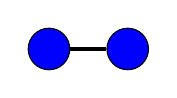
\begin{tikzpicture}[node distance=1cm]
			
			\node[vertex]	(A)	{};
			\node[vertex]	(B) [right of=A]{};
			
			\path[pstyle] (A) edge node {} (B);
			
			\end{tikzpicture}
		\end{column}
		\begin{column}{0.33\textwidth}<+(1)->
			\centering
			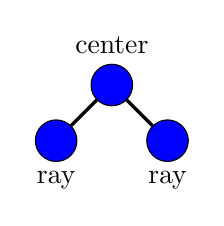
\begin{tikzpicture}[node distance=1cm]
			
			\node[vertex,label=above:{center}]	(A)	{};
			\node[vertex,label=below:{ray}]		(B) [below right of=A]{};
			\node[vertex,label=below:{ray}]		(C) [below left of=A]{};
			
			\path[pstyle]
			(A) edge node {} (B)
			(A) edge node {} (C);
			
			\end{tikzpicture}
		\end{column}
		\begin{column}{0.33\textwidth}<+(1)->
			\centering
			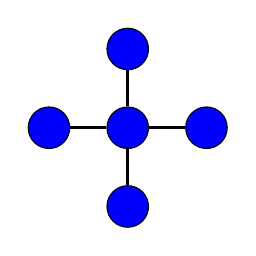
\begin{tikzpicture}[node distance=1cm]
			
			\node[vertex]	(A)	{};
			\node[vertex]	(B) [right of=A]{};
			\node[vertex]	(C) [left of=A]{};
			\node[vertex]	(D) [below of=A]{};
			\node[vertex]	(E) [above of=A]{};
			
			\path[pstyle] 
			(A) edge node {} (B)
			(A) edge node {} (C)
			(A) edge node {} (D)
			(A) edge node {} (E);
			
			\end{tikzpicture}
		\end{column}
	\end{columns}
	
\end{Examples}

\end{frame}



\begin{frame}{Spanning Star Forest Problem}
	\begin{block}{Definition}
		Given a graph $G$ decide whether it has a \emph{Spanning Star Forest}.
	\end{block}
\end{frame}

\begin{frame}{Example}
	\centering
	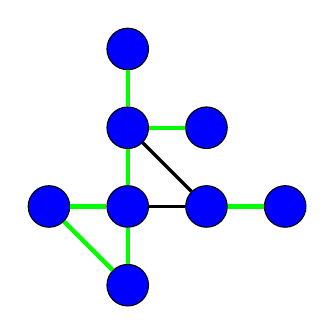
\begin{tikzpicture}[node distance=1cm]
		
		\node[vertex]	(A)	{};
		\node[vertex]	(B) [below of=A]{};
		\node[vertex]	(C) [right of=B]{};
		\node[vertex]	(D) [below of=B]{};
		\node[vertex]	(E) [left of=D]{};
		\node[vertex]	(F) [right of=D]{};
		\node[vertex]	(G) [right of=F]{};
		\node[vertex]	(H) [below of=D]{};
		
		\path[pstyle]<1->
		(A) edge node {} (B)
		(B) edge node {} (C)
		(B) edge node {} (D)
		(B) edge node {} (F)
		(D) edge node {} (E)
		(D) edge node {} (H)
		(D) edge node {} (F)
		(F) edge node {} (G)
		(E) edge node {} (H);
		
		\path[highlight, green]<2>
		(A) edge node {} (B)
		(B) edge node {} (C)
		(B) edge node {} (D)
		(E) edge node {} (H)
		(F) edge node {} (G);
		
		\path[highlight, green]<3>
		(A) edge node {} (B)
		(B) edge node {} (C)
		(D) edge node {} (E)
		(D) edge node {} (H)
		(F) edge node {} (G);
	
	\end{tikzpicture}
\end{frame}

\begin{frame}[t]{Spanning Star Forest Problem}
	\begin{block}{Lemma }
		$G$ contains a Spanning Star Forest if and only if it does not contain any isolated vertices.
	\end{block}
	
	\setlength{\leftmargini}{2pt}
	\begin{columns}[t]
		\begin{column}{0.5\textwidth}
			\begin{itemize}[<+(1)->]
				\item[] \textbf{Forward implication}.
				\item[] Let $S$ - Spanning Star Forest of $G$.
				\item[] Every vertex belongs to a star.
				\item[] Every star has at least 2 vertices.
				\item[] $G$ has no isolated vertices.
			\end{itemize}
		\end{column}
		\begin{column}{0.5\textwidth}
			\begin{itemize}[<+(1)->]
				\item[] \textbf{Backward implication.}
				\item[] Proof on the board.
			\end{itemize}
		\end{column}
	\end{columns}
	
	\vfill
	
	\begin{block}<+(1)>{Corollary}
		\emph{Spanning Star Forest} problem can be solved in \textbf{linear time}.
	\end{block}
	
\end{frame}

\begin{frame}[t]{Minimal Spanning Star Forest}

\begin{block}{Minimal Spanning Star Forest}
	Given a pair $(G,k)$ decide whether there exists a Spanning Star Forest of at most $\mathbf{k}$.
\end{block}

\bigskip

\begin{block}{Dominating Set}<+(1)->
	Given a pair $(G,k)$ find a set $D \subseteq V(G)$ such that $|D| \leq k$ and every node is either in $D$ or adjacent to $D$.
\end{block}

\end{frame}

\begin{frame}{Examples}
	\small
	\begin{columns}
		\begin{column}{0.5\textwidth}
			\centering
			$(G,3)$ for Dominating Set.
			\\ \bigskip
			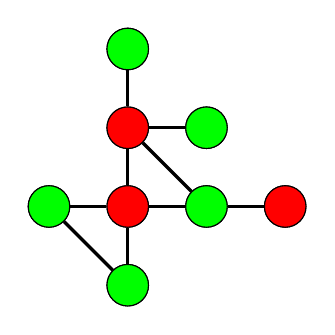
\begin{tikzpicture}[node distance=1cm]
				\tikzstyle{dominating} = [fill=red]
				\tikzstyle{dominated} = [fill=green]
				
				\node[vertex]	(A)	{};
				\node[vertex]	(B) [below of=A]{};
				\node[vertex]	(C) [right of=B]{};
				\node[vertex]	(D) [below of=B]{};
				\node[vertex]	(E) [left of=D]{};
				\node[vertex]	(F) [right of=D]{};
				\node[vertex]	(G) [right of=F]{};
				\node[vertex]	(H) [below of=D]{};
				
				\path[pstyle]
				(A) edge node {} (B)
				(B) edge node {} (C)
				(B) edge node {} (D)
				(B) edge node {} (F)
				(D) edge node {} (E)
				(D) edge node {} (H)
				(D) edge node {} (F)
				(F) edge node {} (G)
				(E) edge node {} (H);
				
				\onslide<2->{
					\node[vertex,dominated]	(A)	{};
					\node[vertex,dominating]	(B) [below of=A]{};
					\node[vertex,dominated]	(C) [right of=B]{};
					\node[vertex,dominating]	(D) [below of=B]{};
					\node[vertex,dominated]	(E) [left of=D]{};
					\node[vertex,dominated]	(F) [right of=D]{};
					\node[vertex,dominating]	(G) [right of=F]{};
					\node[vertex,dominated]	(H) [below of=D]{};
				}
			
			\end{tikzpicture}
		\end{column}
		\begin{column}{0.5\textwidth}
			\centering
			$(G,3)$ for Minimal Spanning Star Forest.
			\\ \bigskip
			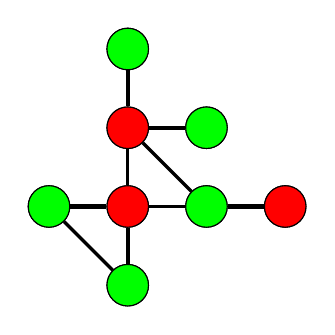
\begin{tikzpicture}[node distance=1cm]
				\tikzstyle{dominating} = [fill=red]
				\tikzstyle{dominated} = [fill=green]
				
				\onslide<-2>{
					\node[vertex]	(A)	{};
					\node[vertex]	(B) [below of=A]{};
					\node[vertex]	(C) [right of=B]{};
					\node[vertex]	(D) [below of=B]{};
					\node[vertex]	(E) [left of=D]{};
					\node[vertex]	(F) [right of=D]{};
					\node[vertex]	(G) [right of=F]{};
					\node[vertex]	(H) [below of=D]{};
				}
				
				\path[pstyle]<-2>
					(A) edge node {} (B)
					(B) edge node {} (C)
					(B) edge node {} (D)
					(B) edge node {} (F)
					(D) edge node {} (E)
					(D) edge node {} (H)
					(D) edge node {} (F)
					(F) edge node {} (G)
					(E) edge node {} (H);
				
				\onslide<3->{
					\node[vertex,dominated]	(A)	{};
					\node[vertex,dominating]	(B) [below of=A]{};
					\node[vertex,dominated]	(C) [right of=B]{};
					\node[vertex,dominating]	(D) [below of=B]{};
					\node[vertex,dominated]	(E) [left of=D]{};
					\node[vertex,dominated]	(F) [right of=D]{};
					\node[vertex,dominating]	(G) [right of=F]{};
					\node[vertex,dominated]	(H) [below of=D]{};
				}
			
				\path[highlight]<3->
					(A) edge node {} (B)
					(B) edge node {} (C)
					(D) edge node {} (E)
					(D) edge node {} (H)
					(F) edge node {} (G);
			\end{tikzpicture}
		\end{column}
	\end{columns}
	\vfill
	\begin{block}{Observation}<+(3)->
		There is a relationship between:
		\setlength{\leftmargini}{20pt}
		\begin{itemize}[<+(3)->]
			\item \textbf{Centers} and \textbf{dominating} vertices.
			\item \textbf{Rays} and \textbf{dominated} vertices.
		\end{itemize}
	\end{block}
\end{frame}

\begin{frame}[t]{Minimal Spanning Star Forest is NP-complete}

	\begin{block}{Theorem}
		Minimal Spanning Star Forest is NP-complete.
	\end{block}
	\bigskip
	\setlength{\leftmargini}{2pt}
	\begin{itemize}[<+(1)->]
		\item[] \textbf{Construction}.
		\item[] Replace every isolated vertex $\mathbf{v}$ with an isolated edge $\mathbf{(v,v')}$.
	\end{itemize}

	\bigskip

	\begin{Lemma}<+(1)->
		$(G,k)$ has a solution if and only if $(G',k)$ has one.
	\end{Lemma}
	
	\onslide<+(1)-> {Proof on the board.}
\end{frame}

\begin{frame}[t]{Reverse reduction}
	\begin{block}{Construction}	
		\begin{equation*}
		(G',k') =
		\begin{cases}
			(G,0), & \text{if } G \text{ contains an isolated vertex}. \\
			(G,k), & \text{otherwise.}
		\end{cases}
		\end{equation*}
	\end{block}
		
	\begin{Lemma}<+(1)->
		$(G,k)$ has a solution if and only if $(G',k)$ has one.
	\end{Lemma}	

	\vfill

	\begin{block}<+(1)->{Corollary}
		Dominating Set and Minimal Spanning Star Forest are interreductible.
	\end{block}

\end{frame}

\begin{frame}[t]{Transfering theorems}

	\begin{block}<+->{Theorem}
		Unless SETH fails, there is no algorithm solving Dominating Set in time $\mathcal{O}^*(n^{k-\epsilon})$ for $\epsilon > 0$.
	\end{block}
	\begin{itemize}[<+->]
		\item[] The theorem is also true for Minimal Spanning Star Forest.
		\bigskip
		\item[] \textbf{Proof}.
		\item[] Suppose contrary, $\mathcal{A}$ is the algorithm.
		\item[] $(G,k)$ - Dominating Set instance.
		\item[] $(G',k)$ - Minimal Spanning Star Forest instance
		\item[] Apply algorithm $\mathcal{A}$. 
		\item[] \textbf{Contradiction}.
		
	\end{itemize}
\end{frame}

\begin{frame}[t]{Spanning Star Forest Extension Problem}
	\begin{block}{Definition}
		Given a graph $G$ and a set of \textbf{forced edges} $M \subseteq E(G)$, find a Spanning Star Forest $S$ such that $M \subseteq E(S)$.\\
	\end{block}

	\bigskip
	
	\begin{columns}
		\begin{column}<+(1)->[t]{0.5\textwidth}
			\centering
			\textcolor{red}{$F = V(M)$} \\
			\textcolor{green}{$R = V \setminus F$} \\
		\end{column}
		\begin{column}{0.5\textwidth}
			\centering
			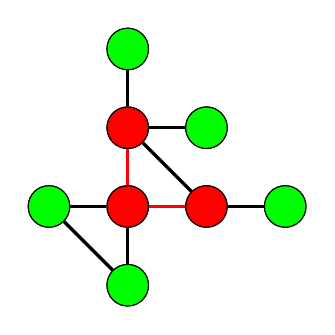
\begin{tikzpicture}<.->[node distance=1cm]
			
			\tikzstyle{state}=[fill=blue,shape=circle]
			
			\node[vertex]	(A)	{};
			\node[vertex]	(B) [below of=A]{};
			\node[vertex]	(C) [right of=B]{};
			\node[vertex]	(D) [below of=B]{};
			\node[vertex]	(E) [left of=D]{};
			\node[vertex]	(F) [right of=D]{};
			\node[vertex]	(G) [right of=F]{};
			\node[vertex]	(H) [below of=D]{};
			
			\path[pstyle]
			(A) edge node {} (B)
			(B) edge node {} (C)
			(B) edge node {} (D)
			(B) edge node {} (F)
			(D) edge node {} (E)
			(D) edge node {} (H)
			(E) edge node {} (H)
			(F) edge node {} (G);
			
			\path[pstyle, red]
			(B) edge node {} (D)
			(D) edge node {} (F);
			
			\onslide<+-> {
				\node[vertex,fill=red]	(B) [below of=A]{};
				\node[vertex,fill=red]	(D) [below of=B]{};
				\node[vertex,fill=red]	(F) [right of=D]{};
			}
			\onslide<.-> {
				\node[vertex,fill=green]	(A)	{};
				\node[vertex,fill=green]	(C) [right of=B]{};
				\node[vertex,fill=green]	(E) [left of=D]{};
				\node[vertex,fill=green]	(G) [right of=F]{};
				\node[vertex,fill=green]	(H) [below of=D]{};
			}
			
			\end{tikzpicture}
		\end{column}
	\end{columns}
	
\end{frame}

\begin{frame}[t]{Instance normalization}
	\setlength{\leftmargini}{25pt}
	\begin{itemize}[<+->]
		\item[(R1)] Isolated vertex $\rightarrow$ no instance.
		\item[(R2)] $G[M]$ not a Star Forest $\rightarrow$ no instance.
		\item[(R3)] $M$ has a star $S$ of size $\geq 3$ $\rightarrow$ remove rays' edges and contract rays.
	\end{itemize}
	\vfill
	\begin{block}<+->{Corollary}
		After exhaustive application of the R3, $M$ is a matching.
	\end{block}
\end{frame}

\begin{frame}[t]{Instance normalization 2}
	\onslide<+-> {
		\setlength{\leftmargini}{2pt}
		\begin{itemize}[<+->]
			\item[] {
				\begin{color}{red}
					$G_{NP}$
				\end{color}
				$= \{v: v \in F \text{ or $v$ is isolated in } G \setminus F\}$
			}
			\item[] {
				\begin{color}{green}
					$G_P$
				\end{color}
				$ = G \setminus G_{NP}$
			}
		\end{itemize}
	}
	\vfill
	\onslide<+->{
		\def\lastx{A}
		\centering
		\begin{tikzpicture}[node distance=2cm]
		
			\node[vertex] (A){};
			
			\foreach \x [remember=\x as \lastx] in {B,...,F} {
				\node[vertex]	(\x)	[right of=\lastx]		{};
			};
			
			\foreach \x in {A,B,D,E} {
				\node[vertex] (\x\x)	[above right of=\x]	{};
			}
			
			\node[vertex] (AAA) [above right of=AA] {};
			
			\path[iso]
			(A) edge node {} (B)
			(C) edge node {} (D)
			(E) edge node {} (F);
			
			\path[pstyle]
			(AA) edge node {} (AAA)
			(BB) edge node {} (AAA)
			(BB) edge node {} (DD)
			(EE) edge node {} (E)
			(DD) edge node {} (E)
			(DD) edge node {} (D)
			(AA) edge node {} (A)
			(AA) edge node {} (B)
			(AA) edge node {} (C)
			(BB) edge node {} (E)
			(BB) edge node {} (D)
			(BB) edge node {} (C);
			
			\only<+->{
				\node[vertex,fill=red] (A){};
				\def\lastx{A}
				\foreach \x [remember=\x as \lastx] in {B,...,F} {
					\node[vertex,fill=red] (\x) [right of=\lastx] {};
				};
				
				\foreach \x in {A,B,D} {
					\node[vertex,fill=green] (\x\x)	[above right of=\x]	{};
				}
				
				\node[vertex,fill=green] (AAA) [above right of=AA] {};
				\node[vertex,fill=red] (EE) [above right of=E] {};
			}
		
		
		\end{tikzpicture}
	} 
	
	\bigskip

	\begin{block}<+->{Corollary}
		$G_P$ has always a solution.
	\end{block}
\end{frame}

\begin{frame}[t]{Instance normalization 2}
	\begin{itemize}
		\item[] {
			\begin{color}{red}
				$G_{NP}$
			\end{color}
			$= \{v: v \in F \text{ or $v$ is isolated in } G \setminus F\}$
		}
		\item[] {
			\begin{color}{green}
				$G_P$
			\end{color}
			$ = G \setminus G_{NP}$
		}
	\end{itemize}
	\begin{Lemma}<+(1)->
		$(G,M)$ has a solution if and only if $(G_{NP},M)$ has one.
	\end{Lemma}
	\begin{columns}[t]
		\begin{column}{0.5\textwidth}
			\begin{itemize}[<+(1)->]
				\item[] \textbf{Backward implication}.
				\item[] Let $S$ be a solution for $G_{NP}$.
				\item[] Partition $G$ into $(G_P, G_{NP})$.
				\item[] Find a solution $S'$ for $G_P$.
				\item[] $S \cup S'$ is a solution for $G$.
			\end{itemize}
		\end{column}
		\begin{column}{0.5\textwidth}
			\begin{itemize}[<+(1)->]
				\item[] \textbf{Forward implication}.
				\item[] Proof on the board.
			\end{itemize}
		\end{column}
	\end{columns}
	
\end{frame}

\begin{frame}[t]{Reduction Rules}
	\setlength{\leftmargini}{25pt}
	\begin{itemize}
		\item[(R1)] Isolated vertex $\rightarrow$ no instance.
		\item[(R2)] $G[M]$ not a Star Forest $\rightarrow$ no instance.
		\item[(R3)] $M$ has a star $S$ of size $\geq 3$ $\rightarrow$ remove rays' edges and contract rays.
		\item[(R4)]<+(1)-> Apply $G = G_{NP}$.
	\end{itemize}
\end{frame}

\begin{frame}[t]{SSFE is NP-complete}
	
	\only<1> {
		\begin{block}{Theorem}
			There exists a reduction from CNF-SAT to SSFE.
		\end{block}
	}
	
	\only<+(1)-5> {
		\small
		\begin{itemize}[<+->]
			\item[] $\phi$ CNF-formula.
			\item[] Variable $\mathbf{x_i}$ $\rightarrow$ \textbf{vertices} $x_i, \neg x_i$ and \textbf{marked edge} $(x_i, \neg x_i)$.
			\item[] Clause $C_i$ $\rightarrow$ \textbf{vertex} $c_i$.
			\item[] literal $\neg x_k$ in clause $c_i$ $\rightarrow$ \textbf{edge}	 $(\neg x_k, c_i)$.
		\end{itemize}
	}
	\only<6-> {
		\begin{block}{Lemma}
			$\phi$ is satisfiable if and only there exists a SSFE.
		\end{block}	
	}
	
	\onslide<2-> {
		\begin{equation*}
			(x_1 \lor x_2 \lor \neg x_4) \land (\neg x_1 \lor x_3 \lor \neg x_5) \land (x_4 \lor x_5 \lor \neg x_1)
		\end{equation*}
		
		\vfill
		\def\lastx{A}
		\begin{tikzpicture}[node distance=1.3cm]
			\onslide<3-> {
				\node[vertex, label=below:{$x_1$}] (A) {};
				\node[vertex, label=below:{$\neg x_1$}] (AA) [right of=A] {};
				\path[pstyle,red] (A) edge node {} (AA);

				\foreach \x [count=\i from 2, remember=\x as \lastx] in {B,...,E} {
					\node[vertex,label=below:{$x_\i$}] (\x)
						[right of=\lastx\lastx] 	{};
					\node[vertex,label=below:{$\neg x_\i$}] (\x\x) 	
						[right of=\x]	{};
					\path[pstyle,red] (\x) edge node {} (\x\x);
				}
			}
			\onslide<4-> {
				\node[vertex, label=above:{$c_1$}] (X) [above= 1.5cm of B] {};
				\node[vertex, label=above:{$c_2$}] (Y) [above= 1.5cm of CC] {};
				\node[vertex, label=above:{$c_3$}] (Z) [above= 1.5cm of DD] {};
			}
		
			\onslide<5-> {
				\path[pstyle]
					(X) edge node {} (A)
					(X) edge node {} (B)
					(X) edge node {} (DD)
					(Y) edge node {} (AA)
					(Y) edge node {} (C)
					(Y) edge node {} (EE)
					(Z) edge node {} (D)
					(Z) edge node {} (E)
					(Z) edge node {} (AA);
			}
			
			 
		\end{tikzpicture}
	}

\end{frame}

\begin{frame}[t]{Reverse reduction}
	\begin{block}{Observation}<only@1>
		There is a relationship between:
		\setlength{\leftmargini}{20pt}
		\begin{itemize}
			\item $\mathbf{M}$ and \textbf{variables}.
			\item $\mathbf{R}$ and \textbf{clauses}.
		\end{itemize}
	\end{block}

	\begin{block}{Theorem}<+(1)->
		There is a reduction from SSFE to CNF-SAT
	\end{block}
	\small
	\begin{itemize}[<+(1)->]
		\item[] \textbf{Construction.}
		\item[] $(G,M)$ $\rightarrow$ SSFE instance
		\item[] $(G',M')$ $\rightarrow$ Exhaustive application of (R1)-(R5).
		\item[] $\phi$ $\rightarrow$ formula of $|M'|$ variables and $|R|$ clauses.
	\end{itemize}

	\begin{block}<+(1)->{Lemma}
		$(G,M)$ has a SSF $\iff$ $\phi$ is satisfiable.
	\end{block}

	\onslide <+-> { Proof on the board.}
\end{frame}

\begin{frame}[t]{Wrap up}
	\begin{block}<+(1)->{Corollary}
		Spanning Star Forest Extension and CNF-SAT are interreductible.
	\end{block}
	\bigskip
	\def\arraystretch{1.5}
	\onslide<+(1)-> {
		\begin{center}
			\begin{tabular}{c|c}
				CNF-SAT & SSFE \\
				\hline
				$n$ variables & $n$ marked edges \\
				\hline
				m clauses & $|R| = m$
			\end{tabular}
		\end{center}
	}
	\vfill
	

	\begin{block}<only@+(1)>{Observation 1}
		Theorems for CNF-SAT paramterized by the number of \textbf{variables} can be transfered to Spanning Star Forest Extension parameterized by the number of \textbf{marked edges}.
	\end{block}
	
	\begin{block}<+(1)->{Observation 2}
		Theorems for CNF-Sat parameterized by the number of \textbf{clauses} can be transfered to Spanning Star Forest Extension paramtereized by $\mathbf{|R|}$.
	\end{block}

\end{frame}

\begin{frame}[t]{Summary}
	\begin{itemize}[<+->]
		\item[] So far we proved that the following problems are interreductible:
	\end{itemize}
	\vfill
	\onslide<+-> {
		\begin{center}
			\def\arraystretch{1.5}
			\begin{tabular}{l|l}
				Dominating Set & Minimal SSF \\				
				\hline
				CNF-Sat $n$ variables & SSFE $|M|$ \\
				\hline
				CNF-Sat $m$ clauses & SSFE $|R|$ \\
			\end{tabular}
		\end{center}
	}
	\vfill
\end{frame}

\begin{frame}[t]{$|M|$ parametrization}
	\only<-2> {
		\begin{block}{Theorem}
			CNF-Sat with $n$ variables doesn't admit any kernel.
		\end{block}
		\onslide<+(1)-> { Consequently, nor does SSFE parameterized by $|M|$. }
	}
	
	
	\begin{block}<+(2)->{Proving nonexistence of a kernel for a problem $\mathcal{P}$}
		Design an algorithm $\mathcal{A}$:
		\begin{enumerate}[<+(2)->]
			\item[] \textbf{Input}: $(x_1,k),(x_2,k),...,(x_p,k)$
			\item[] \textbf{Output}: $(x',k)$.
		\end{enumerate}
		\onslide<+(1)-> {such that:}
		\begin{enumerate}[<+(1)->]
			\item[] \textcolor{blue}{(1)} $k' \leq POLY(k + \log(p))$.
			\item[] \textcolor{blue}{(2)} $(x',k') \in \mathcal{P} \iff (x_i,k) \in \mathcal{P}$ for some $1 \leq i \leq p$
		\end{enumerate}
	\end{block}

	\begin{block}<+(1)->{Theorem}
		SSFE parameterized by $|M|$ doesn't admit a kernel.
	\end{block}

	\onslide<+(1)-> {Proof on the board.}

\end{frame}

\begin{frame}[t]{$|R|$ parametrization}
	\only<-2> {
		\begin{block}{Theorem}<.->
			CNF-Sat parameterized with $m$ clauses has a linear kernel.
		\end{block}
		\onslide<+(1)-> { Consequently, so does SSFE parameterized by $|R|$.}
	}
	\begin{block}<3->{Quadratic kernel}
		If there exists a vertex $v \in R$ such that $deg_G(v) > k$, then remove $v$.
	\end{block}

	\onslide<3-> { Proof on the board. }
	\begin{block}<4->{Corollary}
		After exhaustive application of the rule, an instance contains:
		\begin{itemize}[<+(4)->]
			\item[] $\leq 2k^2$ edges.
			\item[] $\leq k + 2k^2$ vertices.
		\end{itemize}
	\end{block}
\end{frame}

\begin{frame}[t]{SSFE parameterized by $tw(G)$}
	\small
	\textbf{Dynamic table}. $dp[t, f]$ where $t$ is node from a tree decomposition and $f:X_t \rightarrow \{true, false\}$ defined as follows:
	\onslide<+(1)->{
		\begin{align*}
			f(v) =& \begin{cases}
				true, & \text{$v \in F$ and $v$ is a center.} \\
				true, & \text{$v \in R$ and $v$ is a part of a Star Tree.} \\
				false, &\text{otherwise.}
			\end{cases}\\
		\end{align*}
	}
	\bigskip

	\onslide<+(1)-> { Assume we have everything finished \textbf{except for a join node}. }
\end{frame}

\newcommand\drawpic[3]{
	\begin{tikzpicture}[node distance=2cm]
	
	\node[vertex2,label=below:{$f(w)=#1$}] (A) {w};
	\node[vertex2,label=below:{$f(u)=#2$}] (B) [right of=A] {u};
	\node[vertex2,label=above:{$f(v)=#3$}] (C) [above right of=A] {v};
	
	\path[iso] (A) edge node {} (B);
	\path[highlight] (B) edge node {} (C);
	\end{tikzpicture}
}

\newcommand\nextpicture[6]{
	\only<+(1)>{
		\begin{columns}
			\begin{column}{0.33\textwidth}
				\centering
				\textbf{($t_1$)}\\ \bigskip
				\drawpic{#1}{#2}{#3}
			\end{column}
			\begin{column}{0.33\textwidth}
				\centering
				\textbf{($t_2$)}\\ \bigskip
				\drawpic{#1}{#2}{#4}
			\end{column}
			\begin{column}{0.33\textwidth}
				\centering
				\textbf{($t$)}\\ \bigskip
				\drawpic{#1}{#2}{#5}
			\end{column}
		\end{columns}
		\centering
		\bigskip
		#6
	}
}

\newcommand\badpic[3]{
	\only<+(1)>{
		\vfill
		\begin{columns}
			\begin{column}{0.5\textwidth}
				\centering
				\textbf{$(t_1)$}\\ \bigskip
				
				\begin{tikzpicture}[node distance=2cm]
				
				\node[vertex2,label=below:{$f(w)=#1$}] (A) {w};
				\node[vertex2,label=below:{$f(u)=#2$}] (B) [right of=A] {u};
				\node[vertex2,label=above:{$f(v)=?$}] (C) [above right of=A] {v};
				
				\path[iso] (A) edge node {} (B);
				\path[highlight] (B) edge node {} (C);
				\end{tikzpicture}
			\end{column}
			\begin{column}{0.5\textwidth}
				\centering
				\textbf{$(t_2)$}\\ \bigskip
				
				\begin{tikzpicture}[node distance=2cm]
				
				\node[vertex2,label=below:{$f(w)=#2$}] (A) {w};
				\node[vertex2,label=below:{$f(u)=#1$}] (B) [right of=A] {u};
				\node[vertex2,label=above:{$f(v)=?$}] (C) [above right of=A] {v};
				
				\path[iso] (A) edge node {} (B);
				\path[highlight] (B) edge node {} (C);
				\end{tikzpicture}
			\end{column}
		\end{columns}
		\centering
		\bigskip
		#3
	}
}

\begin{frame}[t]{SSFE parameterized by $tw(G)$}
\small
\textbf{Join nodes $t_1$, $t_2$}
\vfill
\badpic{0}{1}{}
\badpic{1}{0}{$C_1 =$ For every vertex  $v \in (F \cap X_t)$ it holds $f(v)=f_1(v)=f_2(v)$}
\nextpicture{0}{1}{1}{1}{1}{}
\nextpicture{0}{1}{1}{0}{1}{}
\nextpicture{0}{1}{0}{1}{1}{$C_2 =$ For all $v \in R$ it holds $f(v) = f_1(v) \lor f_2(v)$.}
\end{frame}

\begin{frame}[t]{SSFE parameterized by $tw(G)$}
\nextslide{
\begin{equation*}
dp[t,f] = \begin{cases}
\bigvee\limits_{f_1,f_2} dp[t_1,f_1] \land dp[t_2,f_2], &\text{ if $C_1$ and $C_2$ holds.} \\
false, &\text{ otherwise.}
\end{cases}
\end{equation*}
}

\setlength{\leftmargini}{2pt}
\begin{itemize}[<+(1)->]
	\item[] There are $\mathbf{2^{|X_t|}}$ functions. 
	\smallskip
	\item[] \textbf{Naive approach}: Each $f$ in $\mathcal{O}^*(2^{|X_t|})$.
	\smallskip
	\item[] \textbf{Total complexity}: $\mathcal{O}^*(4^{|X_t|})$.
	\bigskip
	\item[] \textbf{Cover product}: all functions $f$ in time $\mathcal{O}^*(2^{|X_t|})$ 
	\bigskip
	\item[] Assuming leaf, introduce and forget are easy:
\end{itemize}

\end{frame}

\begin{frame}[t]{Lower bound}
	\begin{block}{SSFE parameterized by $tw(G)$}
		SSFE parameterized by treewidth can be solved in $\mathcal{O}^*(2^{tw(G)})$.
	\end{block}
	
	\begin{block}<+(1)->{Lower bound}
		Assuming SETH, $\mathcal{O}^*(2^{tw(G)})$ is optimal.
	\end{block}

	\onslide<+-> { Proof on the board.}
\end{frame}

\end{document}
